% ==== Color definitions ====
\definecolor{rank1}{RGB}{255, 190, 128}   % 深橙色：第一名
\definecolor{rank2}{RGB}{255, 210, 160}   % 中橙色：第二名
\definecolor{rank3}{RGB}{255, 230, 190}   % 浅橙色：第三名
\definecolor{baselinebg}{RGB}{245, 245, 245} % baseline背景

% ==== Custom commands ====
\newcommand{\rankone}[1]{\cellcolor{rank1}\textbf{#1}}
\newcommand{\ranktwo}[1]{\cellcolor{rank2}\textbf{#1}}
\newcommand{\rankthree}[1]{\cellcolor{rank3}\textbf{#1}}
\newcommand{\baseline}[1]{\cellcolor{baselinebg}#1}

\section{Experiments}
\label{sec:exp}

\subsection{Implementation Details}
\label{sec:exp_imp}

The MLP of RAP consists of three hidden layers with widths of 32, 32, and 16 neurons, respectively.
We set $\lambda_{\text{dssim}} = 0.2$, $\lambda_{\text{render}} = 1.0$, $\lambda_{\text{prune}} = 1.0$, and $\lambda_{\text{entropy}} = 0.25$ for the loss terms. 
Feature extraction uses $K = 128$ nearest neighbors for local statistics, $B = 250$ bins for the entropy approximation, and a Gaussian kernel width of $\sigma = 0.01$. 
The MLP is trained for 15{,}000 iterations on 10 randomly selected scenes from the DL3DV-10K~\cite{dl3dv} dataset.

We evaluate RAP on the same three benchmarks as the original 3DGS~\cite{3dgs}, including the full set of scenes from Mip-NeRF360~\cite{mip360} (five outdoor and four indoor scenes), two scenes from DeepBlending~\cite{db}, and two scenes from Tanks\&Temples~\cite{tandt}. 
All scenes are trained following the standard 3DGS protocol, using $7/8$ of the views for training and the remaining $1/8$ for testing.

We compare RAP with multiple baselines, including a simple opacity-thresholding heuristic, visibility-based approaches such as LightGaussian~\cite{lightgaussian}, MesonGS~\cite{mesongs}, and EAGLES~\cite{eagles}, and gradient-based approaches such as C3DGS~\cite{c3dgs} and PUP-3DGS~\cite{pup}. 
For rendering-based baselines, importance scores are computed using the training views to ensure a fair comparison under identical conditions.


\subsection{Post-hoc Pruning on Trained 3DGS}
\label{sec:exp1_post_pruning}
We perform post-hoc pruning experiments on pretrained 3DGS representations by retaining a fixed percentage (from 5\% to 95\%) of the Gaussians with the highest predicted importance scores. 

Performance is evaluated by plotting retention-ratio vs. reconstruction-quality curves (PSNR, SSIM, LPIPS) in Fig.~\ref{fig:exp1_rd}. 
Due to space constraints, we report only the average PSNR across the Mip-NeRF360-Outdoor, Mip-NeRF360-Indoor, Deep Blending, and Tanks\&Temples datasets in the main paper; per-scene results and the full set of SSIM and LPIPS metrics are provided in the supplementary material. 

Considering that pruning can be used as part of GS compression, to further quantify pruning efficiency, we compute the BD-Rate (Bjøntegaard Delta Bitrate) inspired by compression research of each method relative to the opacity-based baseline, using the average per-scene storage size as the rate axis. 
This metric provides a compact assessment of rate-distortion behavior across datasets---a lower BD-Rate indicates superior reconstruction quality under comparable storage budgets. 
The summarized results are presented in Table~\ref{tab:exp1_bdbr}.

\label{subsec:post_hoc}
\begin{figure}[t]
  \centering
  % \fbox{\rule{0pt}{2in} \rule{0.9\linewidth}{0pt}}
   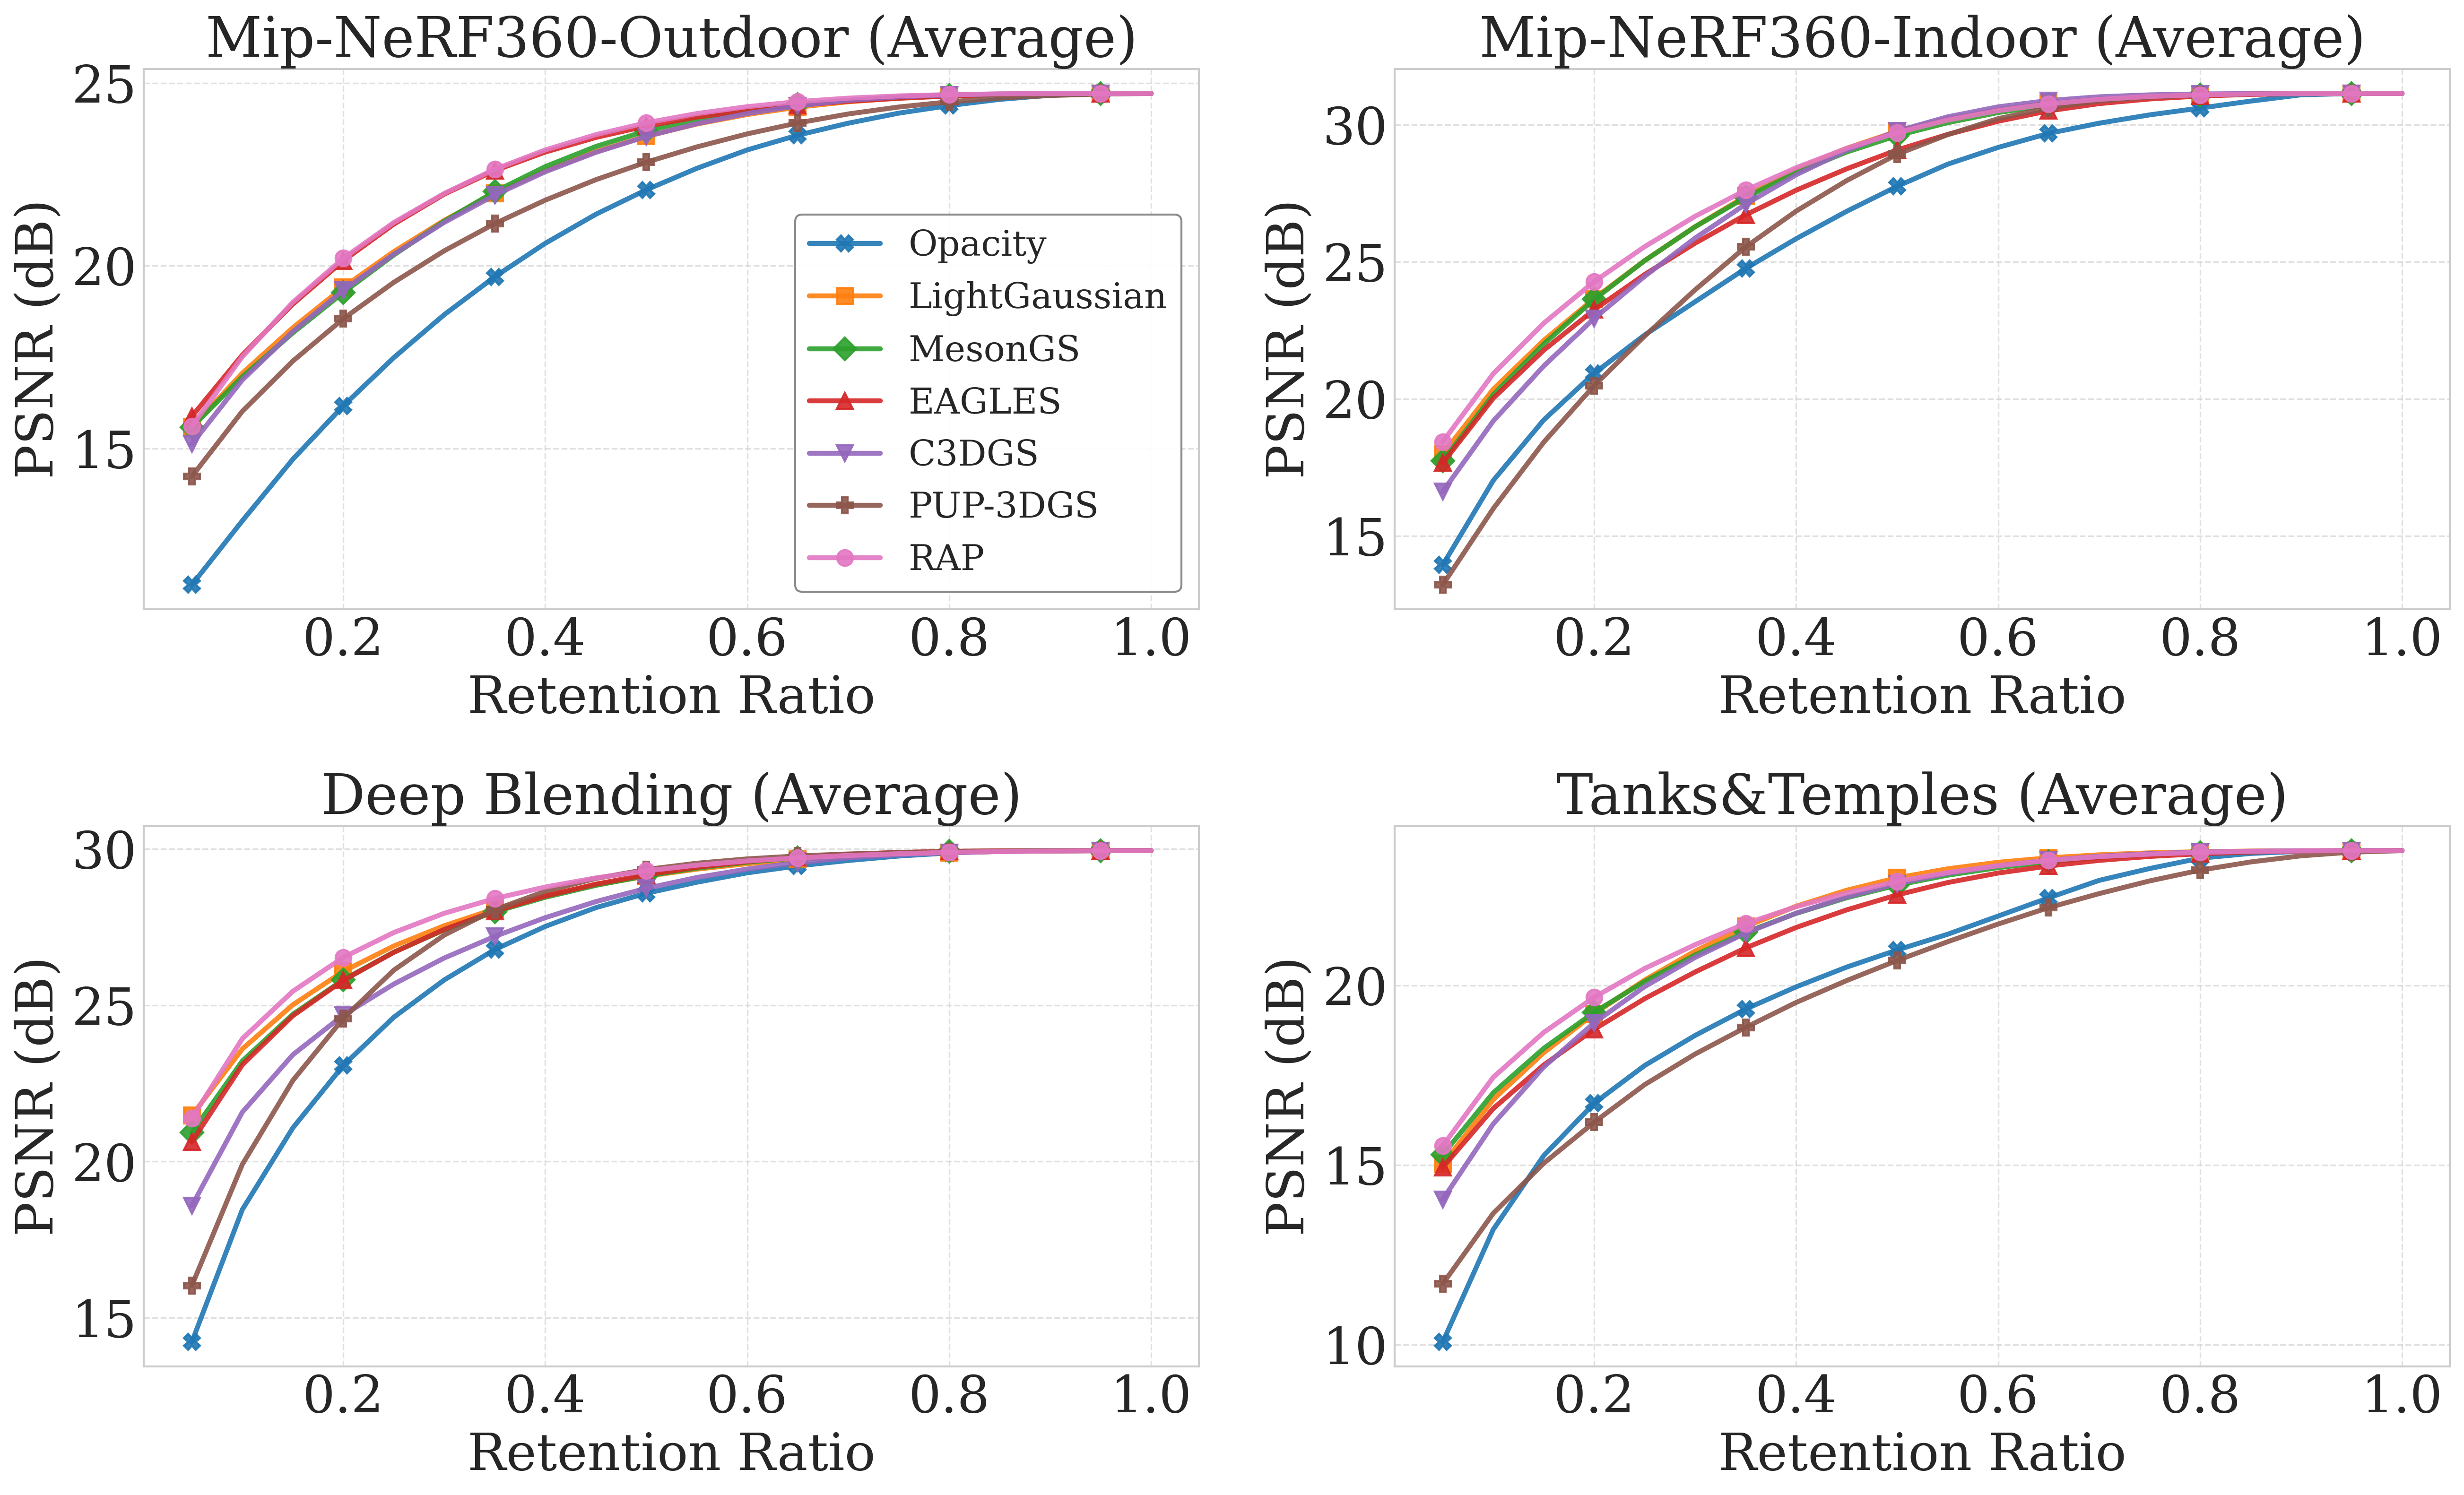
\includegraphics[width=\linewidth]{sec/imgs_main/rd_curve_by_PSNR_baseline_dataset_avg.png}
   \caption{PSNR vs. retention ratio curves. }
   \label{fig:exp1_rd}
   \vspace{-1em}
\end{figure}

\begin{table}[t]
    \centering
    \caption{BD-Rate (\%) comparison of pruning-based Gaussian Splatting methods relative to the opacity baseline. Lower BD-Rate indicates better rate–distortion efficiency}
    \label{tab:exp1_bdbr}
    \resizebox{\columnwidth}{!}{%
    \begin{tabular}{|l|c|c|c|c|c|c|}
    \hline
    \textbf{} & \textbf{LightGS} & \textbf{MesonGS} & \textbf{EAGLES} & \textbf{C3DGS} & \textbf{PUP-3DGS} & \textbf{RAP} \\ \hline
    \textbf{Mip-Outdoor} 
        & \rankthree{-35.21} 
        & -34.89 
        & \ranktwo{-41.28} 
        & -33.77 
        & -22.54 
        & \rankone{-42.63} \\ \hline
    \textbf{Mip-Indoor}  
        & \ranktwo{-31.15} 
        & \rankthree{-30.34} 
        & -24.98 
        & -27.63 
        & -8.70 
        & \rankone{-33.90} \\ \hline
    \textbf{Deep Blending}       
        & \ranktwo{-30.72} 
        & -28.84 
        & \rankthree{-29.87} 
        & -16.28 
        & -19.46 
        & \rankone{-36.76} \\ \hline
    \textbf{Tanks\&Temples}      
        & \ranktwo{-37.98} 
        & \rankthree{-36.12} 
        & -30.01 
        & -34.37 
        & 7.06 
        & \rankone{-40.11} \\ \hline
    \end{tabular}%
    }
    \vspace{-1.5em}
\end{table}
As shown in Fig.~\ref{fig:exp1_rd} and Table~\ref{tab:exp1_bdbr}, our method consistently outperforms prior approaches across all datasets and pruning ratios. 
While the performance gap is relatively small under light pruning (e.g., retention $>$50\%), it becomes increasingly pronounced as pruning becomes more aggressive. 
At a pruning ratio of 60\%, RAP achieves up to a 0.5~dB PSNR gain over competing methods. 
The superiority is further reflected in BD-Rate reductions, with improvements such as $-42.63\%$ on the Mip-NeRF360-Outdoor dataset.


We also observe a notable difference in robustness between visibility-based and gradient-based methods. The former (e.g., LightGaussian, MesonGS, EAGLES) exhibit more consistent performance across datasets, while the latter (e.g., C3DGS, PUP-3DGS) show larger variance. For instance, C3DGS performs comparably on Mip-NeRF360 but suffers over 1 dB drop on Deep Blending. On Tanks\&Temples, PUP-3DGS even underperforms the opacity baseline, with a positive BD-Rate of {+7.06\%}, indicating poor generalization across diverse scenes.

Lastly, we find that when the importance estimation function is sufficiently accurate, up to 40\% of Gaussians can be pruned with negligible degradation in rendering quality. Even at a 60\% pruning rate, the average PSNR drop remains within 2 dB. These results suggest that reliable importance scoring can enable highly compact representations without significantly compromising visual fidelity.

\begin{table}[]
    \centering
    \caption{Importance score computation time (seconds).}
    \label{tab:exp_importance_time}
    \resizebox{\columnwidth}{!}{%
    \begin{tabular}{|l|c|c|c|c|c|c|c|}
    \hline
    \textbf{Dataset} & \textbf{Opacity} & \textbf{LightGS} & \textbf{MesonGS} & \textbf{EAGLES} & \textbf{C3DGS} & \textbf{PUP-3DGS} & \textbf{RAP} \\ \hline
    \textbf{Mip-Outdoor} & \rankone{3.73} & 15.86 & 42.40 & 42.96 & \ranktwo{11.69} & 20.95 & 15.64 \\ \hline
    \textbf{Mip-Indoor}  & \rankone{1.27} & 22.71 & 14.84 & 14.97 & 15.96 & 21.22 & \ranktwo{5.72} \\ \hline
    \textbf{Deep Blending} & \rankone{2.99} & 20.20 & 31.30 & 31.65 & 13.62 & 20.28 & \ranktwo{11.64} \\ \hline
    \textbf{Tanks\&Temples} & \rankone{2.53} & 18.62 & 17.53 & 13.92 & 9.22 & 20.50 & \ranktwo{6.66} \\ \hline
    \end{tabular}%
    }
    \vspace{-1.5em}
\end{table}

Table~\ref{tab:exp_importance_time} reports the computation time for importance score prediction (including point loading and metric computation). 
RAP is among the fastest methods across datasets: it ranks second (behind the trivial opacity baseline) on Mip-NeRF360-Indoor, Deep Blending, and Tanks\&Temples, and third on Mip-NeRF360-Outdoor where C3DGS is slightly faster (11.69\,s vs.\ 15.64\,s for RAP). 
Despite this single exception, RAP consistently outpaces all visibility-based approaches (LightGaussian, MesonGS, EAGLES) by a wide margin, and is generally faster than gradient-based methods (C3DGS, PUP-3DGS). 
This advantage stems from RAP’s feature-driven, rendering-free design, which avoids per-view rasterization and back-propagation; consequently, runtime scales with the number of primitives rather than with the number of training views, enabling efficient deployment across diverse scenes.

\subsection{Pruning-in-the-Loop Training}
\label{sec:exp2_rec_pruning}
To evaluate the potential of integrating pruning directly into the 3DGS generation process, we modify the pipeline to periodically remove redundant Gaussians during optimization. This experiment is motivated by the observation in Sec.~\ref{subsec:post_hoc}, where pruning up to 40\% of Gaussians post-training leads to negligible quality degradation.

Specifically, we embed the pruning strategy into the densification phase: every \textbf{1500} training iterations, we apply a pruning operation to remove the bottom \textbf{40\%} of Gaussians ranked by the importance score predicted by each method are removed. To assess the effectiveness of this integration, we compare the final reconstructions against the standard 3DGS training baseline (without pruning) using four metrics: PSNR, SSIM, LPIPS, and storage size (MB).

\begin{table*}[hbpt]
\centering
\caption{Reconstruction quality and size comparison under integrated pruning (40\% pruning every 1500 iterations).}
\label{tab:exp_reconstruction}
\resizebox{0.9\textwidth}{!}{%
\begin{tabular}{lcccccccccccccccc}
\toprule
\textbf{Method} & \multicolumn{4}{c}{\textbf{MipNeRF360 Outdoor}} & \multicolumn{4}{c}{\textbf{MipNeRF360 Indoor}} & \multicolumn{4}{c}{\textbf{Deep Blending}} & \multicolumn{4}{c}{\textbf{Tanks \& Temples}} \\
\cmidrule(lr){2-5} \cmidrule(lr){6-9} \cmidrule(lr){10-13} \cmidrule(lr){14-17}
& PSNR ↑ & SSIM ↑ & LPIPS ↓ & Size ↓ 
& PSNR ↑ & SSIM ↑ & LPIPS ↓ & Size ↓ 
& PSNR ↑ & SSIM ↑ & LPIPS ↓ & Size ↓ 
& PSNR ↑ & SSIM ↑ & LPIPS ↓ & Size ↓ \\
\midrule
\rowcolor{baselinebg}
3DGS & \baseline{24.688} & \baseline{0.729} & \baseline{0.238} & \baseline{926.895} 
     & \baseline{31.076} & \baseline{0.925} & \baseline{0.186} & \baseline{299.202} 
     & \baseline{29.817} & \baseline{0.907} & \baseline{0.239} & \baseline{586.064} 
     & \baseline{23.734} & \baseline{0.853} & \baseline{0.169} & \baseline{372.036} \\
\midrule
Opacity & 24.550 & 0.718 & 0.275 & 313.657 
        & \rankthree{30.604} & \rankthree{0.912} & 0.216 & 72.176 
        & \ranktwo{29.899} & \rankone{0.910} & \rankone{0.248} & 149.873 
        & \ranktwo{23.674} & \ranktwo{0.842} & \rankthree{0.200} & 118.414 \\

LightGaussian & \ranktwo{24.676} & \rankone{0.728} & \rankone{0.255} & 300.907 
        & \rankone{30.777} & \rankone{0.917} & \rankone{0.205} & 71.676 
        & \rankthree{29.839} & \rankthree{0.908} & \ranktwo{0.249} & 155.207 
        & \rankthree{23.634} & \rankone{0.845} & \rankone{0.191} & 118.048 \\

MesonGS & 24.554 & \rankthree{0.723} & \ranktwo{0.256} & 297.255 
        & 30.173 & \ranktwo{0.914} & \ranktwo{0.207} & 71.587 
        & 29.638 & 0.904 & 0.254 & 154.137 
        & 23.541 & \rankthree{0.839} & \ranktwo{0.197} & 115.922 \\

EAGLES & 24.520 & 0.722 & \ranktwo{0.256} & \rankthree{295.899} 
       & 29.801 & 0.911 & \rankthree{0.210} & 71.356 
       & 29.551 & 0.904 & 0.254 & 154.352 
       & 23.212 & 0.834 & 0.202 & \rankthree{113.500} \\

C3DGS & \rankthree{24.638} & \rankthree{0.723} & 0.262 & 303.820 
      & 30.271 & \rankthree{0.912} & 0.212 & \ranktwo{67.821} 
      & 29.739 & 0.905 & 0.258 & \rankone{139.431} 
      & 23.421 & 0.836 & 0.205 & 115.941 \\

PUP-3DGS & 24.328 & 0.714 & \rankthree{0.261} & \rankone{281.821} 
         & 29.422 & 0.909 & 0.212 & \rankthree{70.056} 
         & 29.699 & \rankthree{0.908} & \rankone{0.248} & \ranktwo{145.294} 
         & 22.365 & 0.816 & 0.215 & \rankone{107.662} \\

RAP & \rankone{24.709} & \ranktwo{0.726} & 0.263 & \ranktwo{285.067} 
    & \ranktwo{30.696} & 0.911 & 0.218 & \rankone{67.804} 
    & \rankone{29.913} & \ranktwo{0.909} & \rankthree{0.252} & \rankthree{147.250} 
    & \rankone{23.774} & \ranktwo{0.842} & 0.201 & \ranktwo{113.236} \\
\bottomrule
\end{tabular}
}
\vspace{-1.5em}
\end{table*}

The results, summarized in Table~\ref{tab:exp_reconstruction}, show that integrating pruning introduces negligible quality degradation while achieving substantial model size reduction. The reconstructed Gaussian sets are only about one-third to one-fifth the size of the original models, with similar performance across methods. The proposed RAP reports higher PSNRs than vanilla GS on MipNeRF360 Outdoor, Deep Blending, and Tanks \& Temples, while other approaches generally give a PSNR drop of 0.3--0.5~dB. It indicates that the proposed RAP can facilitate the optimization process via accurately removing redundant primitives, as well as resulting in a better convergence direction. We found that all the pruning methods demonstrate a PSNR decrease on MipNeRF360 Indoor, and an obviously larger drop (around 1.5~dB) is observed with PUP-3DGS and EAGLES, revealing that this dataset is more challenging than the others.   

On the other hand, directly using opacity as the pruning score also yields competitive PSNR results---ranking third on MipNeRF360-Outdoor and second on Deep~Blending and Tanks\&Temples. This can be explained by the densification behavior: when pruning is sub-optimal, the densification process tends to over-generate new Gaussians to compensate, resulting in more primitives but still competitive reconstruction quality, which can be found by the model size of ``Opacity".

\subsection{Integration with MPEG GSC}

\begin{figure}[t]
  \centering
  \begin{subfigure}{0.48\linewidth}
    \centering
    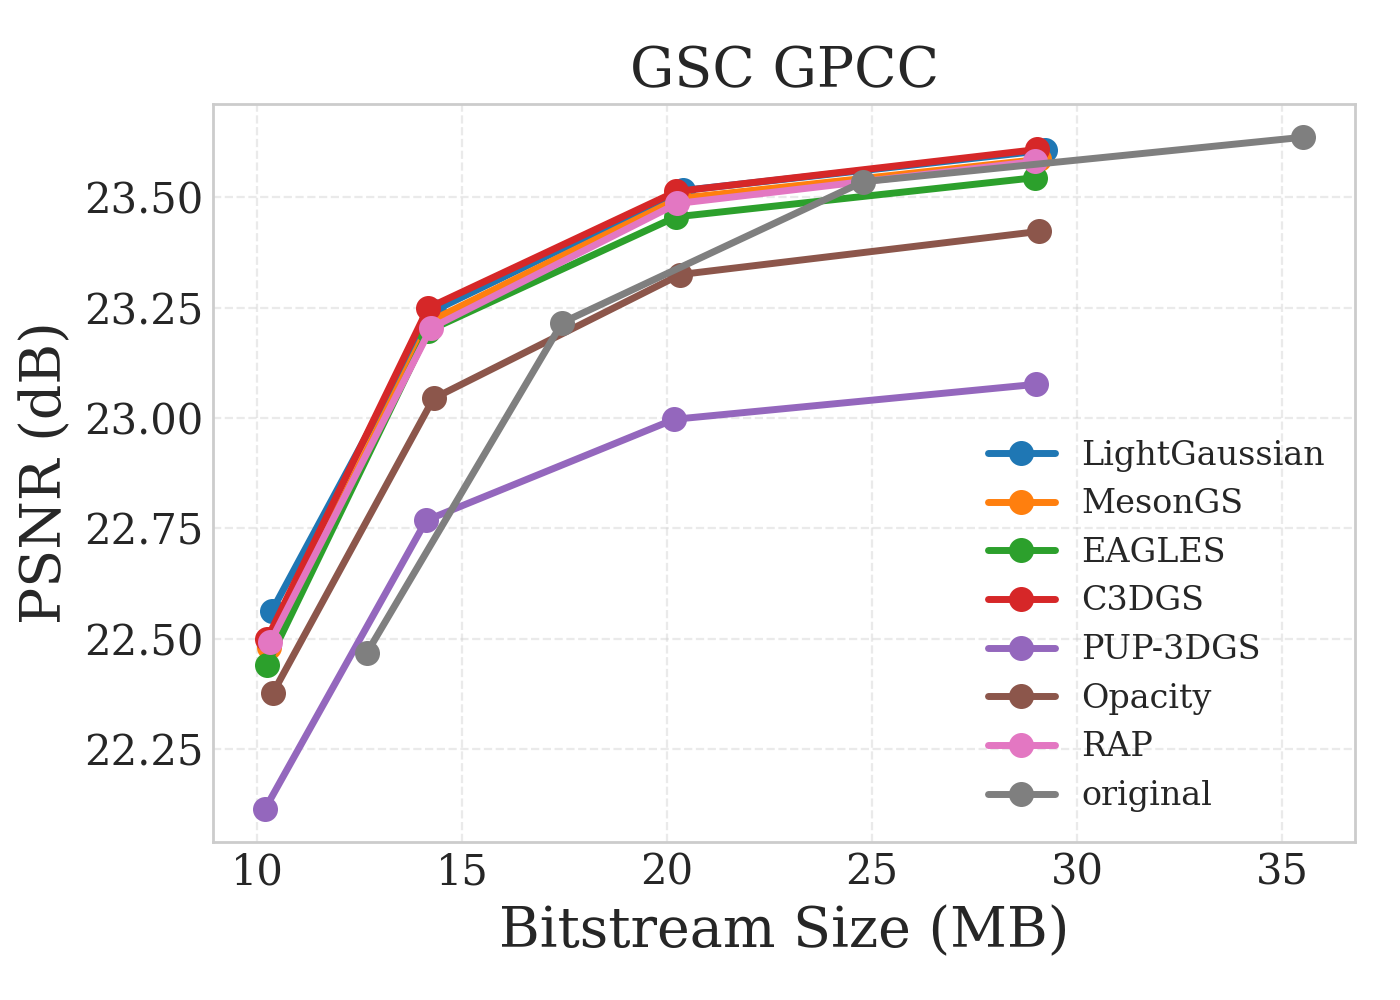
\includegraphics[width=\linewidth]{sec/imgs_main/gsc_gpcc_avg.png}
    \caption{GSC GPCC}
    \label{fig:gsc_gpcc_avg}
  \end{subfigure}
  \hfill
  \begin{subfigure}{0.48\linewidth}
    \centering
    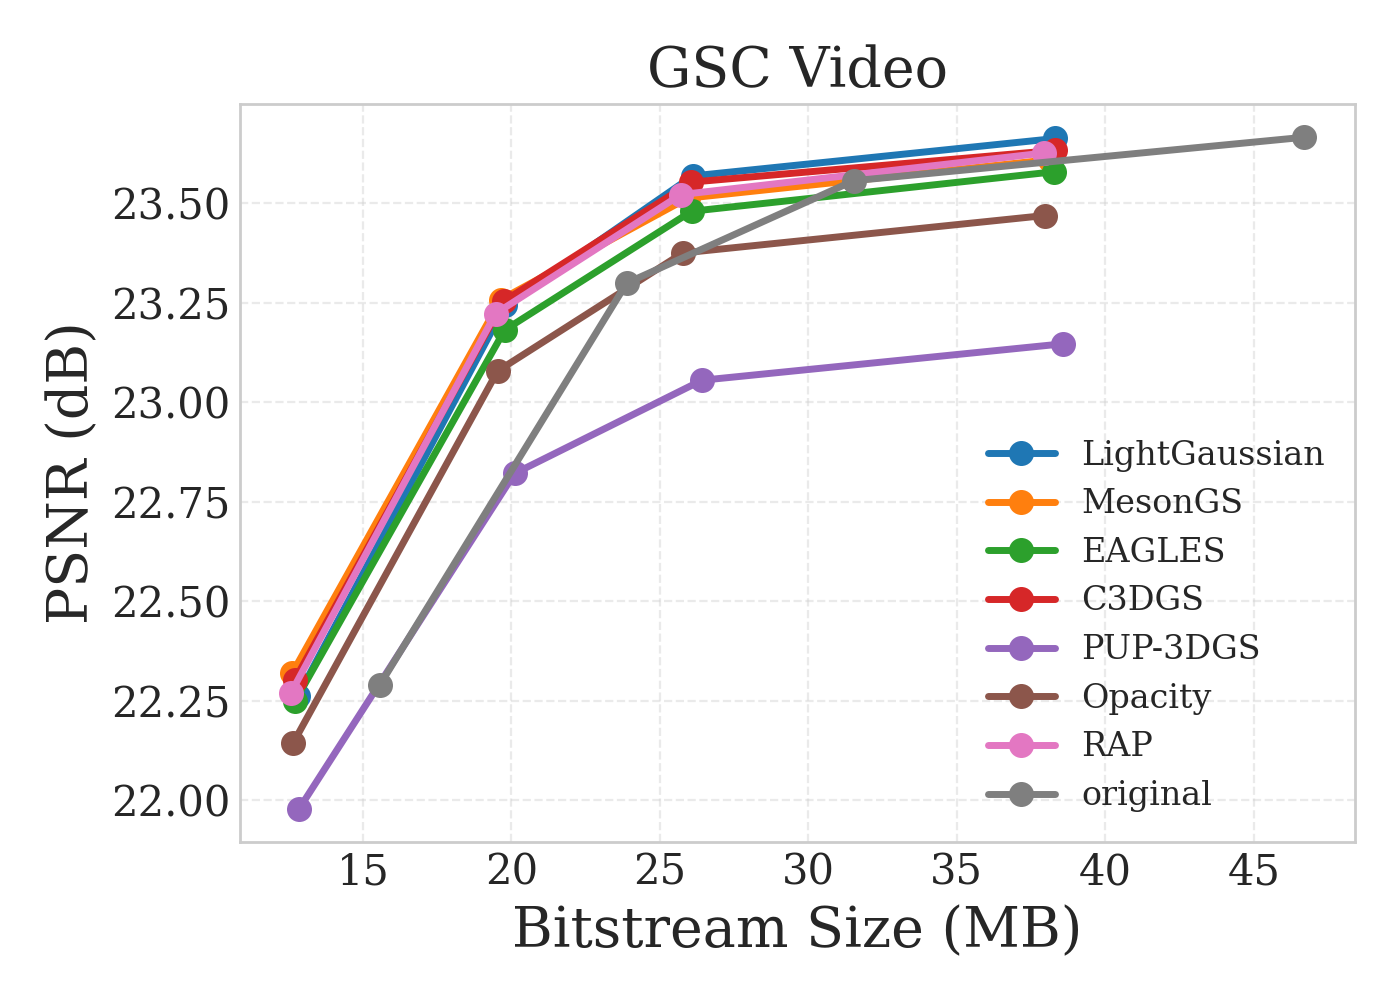
\includegraphics[width=\linewidth]{sec/imgs_main/gsc_video_avg.png}
    \caption{GSC Video}
    \label{fig:gsc_video_avg}
  \end{subfigure}

  \caption{
    R-D curves for GSC with 20\% pruning
  }
  \label{fig:gsc_avg}
  \vspace{-1.5em}
\end{figure}
To evaluate whether importance-guided pruning benefits downstream compression, 
we integrate the pruning step as a pre-processing module into both branches of 
MPEG Gaussian Splat Coding (GSC)~\cite{mpeg_gsc}: the G-PCC–based~\cite{gpcc} 
and the video-based pipeline~\cite{gscodec_studio}. 
For each scene, 20\% of the Gaussians are removed according to the predicted importance  scores, and the remaining primitives are encoded using identical codec settings at four 
rate points. Rate–distortion (R-D) curves are reported in Fig.~\ref{fig:gsc_avg}. Importance-guided pruning consistently improves coding efficiency for both branches. Most pruning methods achieve \textbf{15--20\%} BD-Rate gains.
RAP remains in the top performance band, indicating strong generalization under diverse scene conditions.
In contrast, PUP-3DGS and simple opacity thresholding exhibit unstable behavior across datasets. 
 
Although the G-PCC--based pipeline attains higher PSNR at lower bitrates than the video-based one, both benefit substantially from pre-pruning. 
Overall, these results show that effective importance-guided pruning produces compact yet encoder-friendly Gaussian sets and significantly boosts GSC coding efficiency regardless of the codec design.


\subsection{Ablation Studies}
\label{sec:abla}
\begin{figure}[t]
  \centering

  \begin{subfigure}{0.48\linewidth}
    \centering
    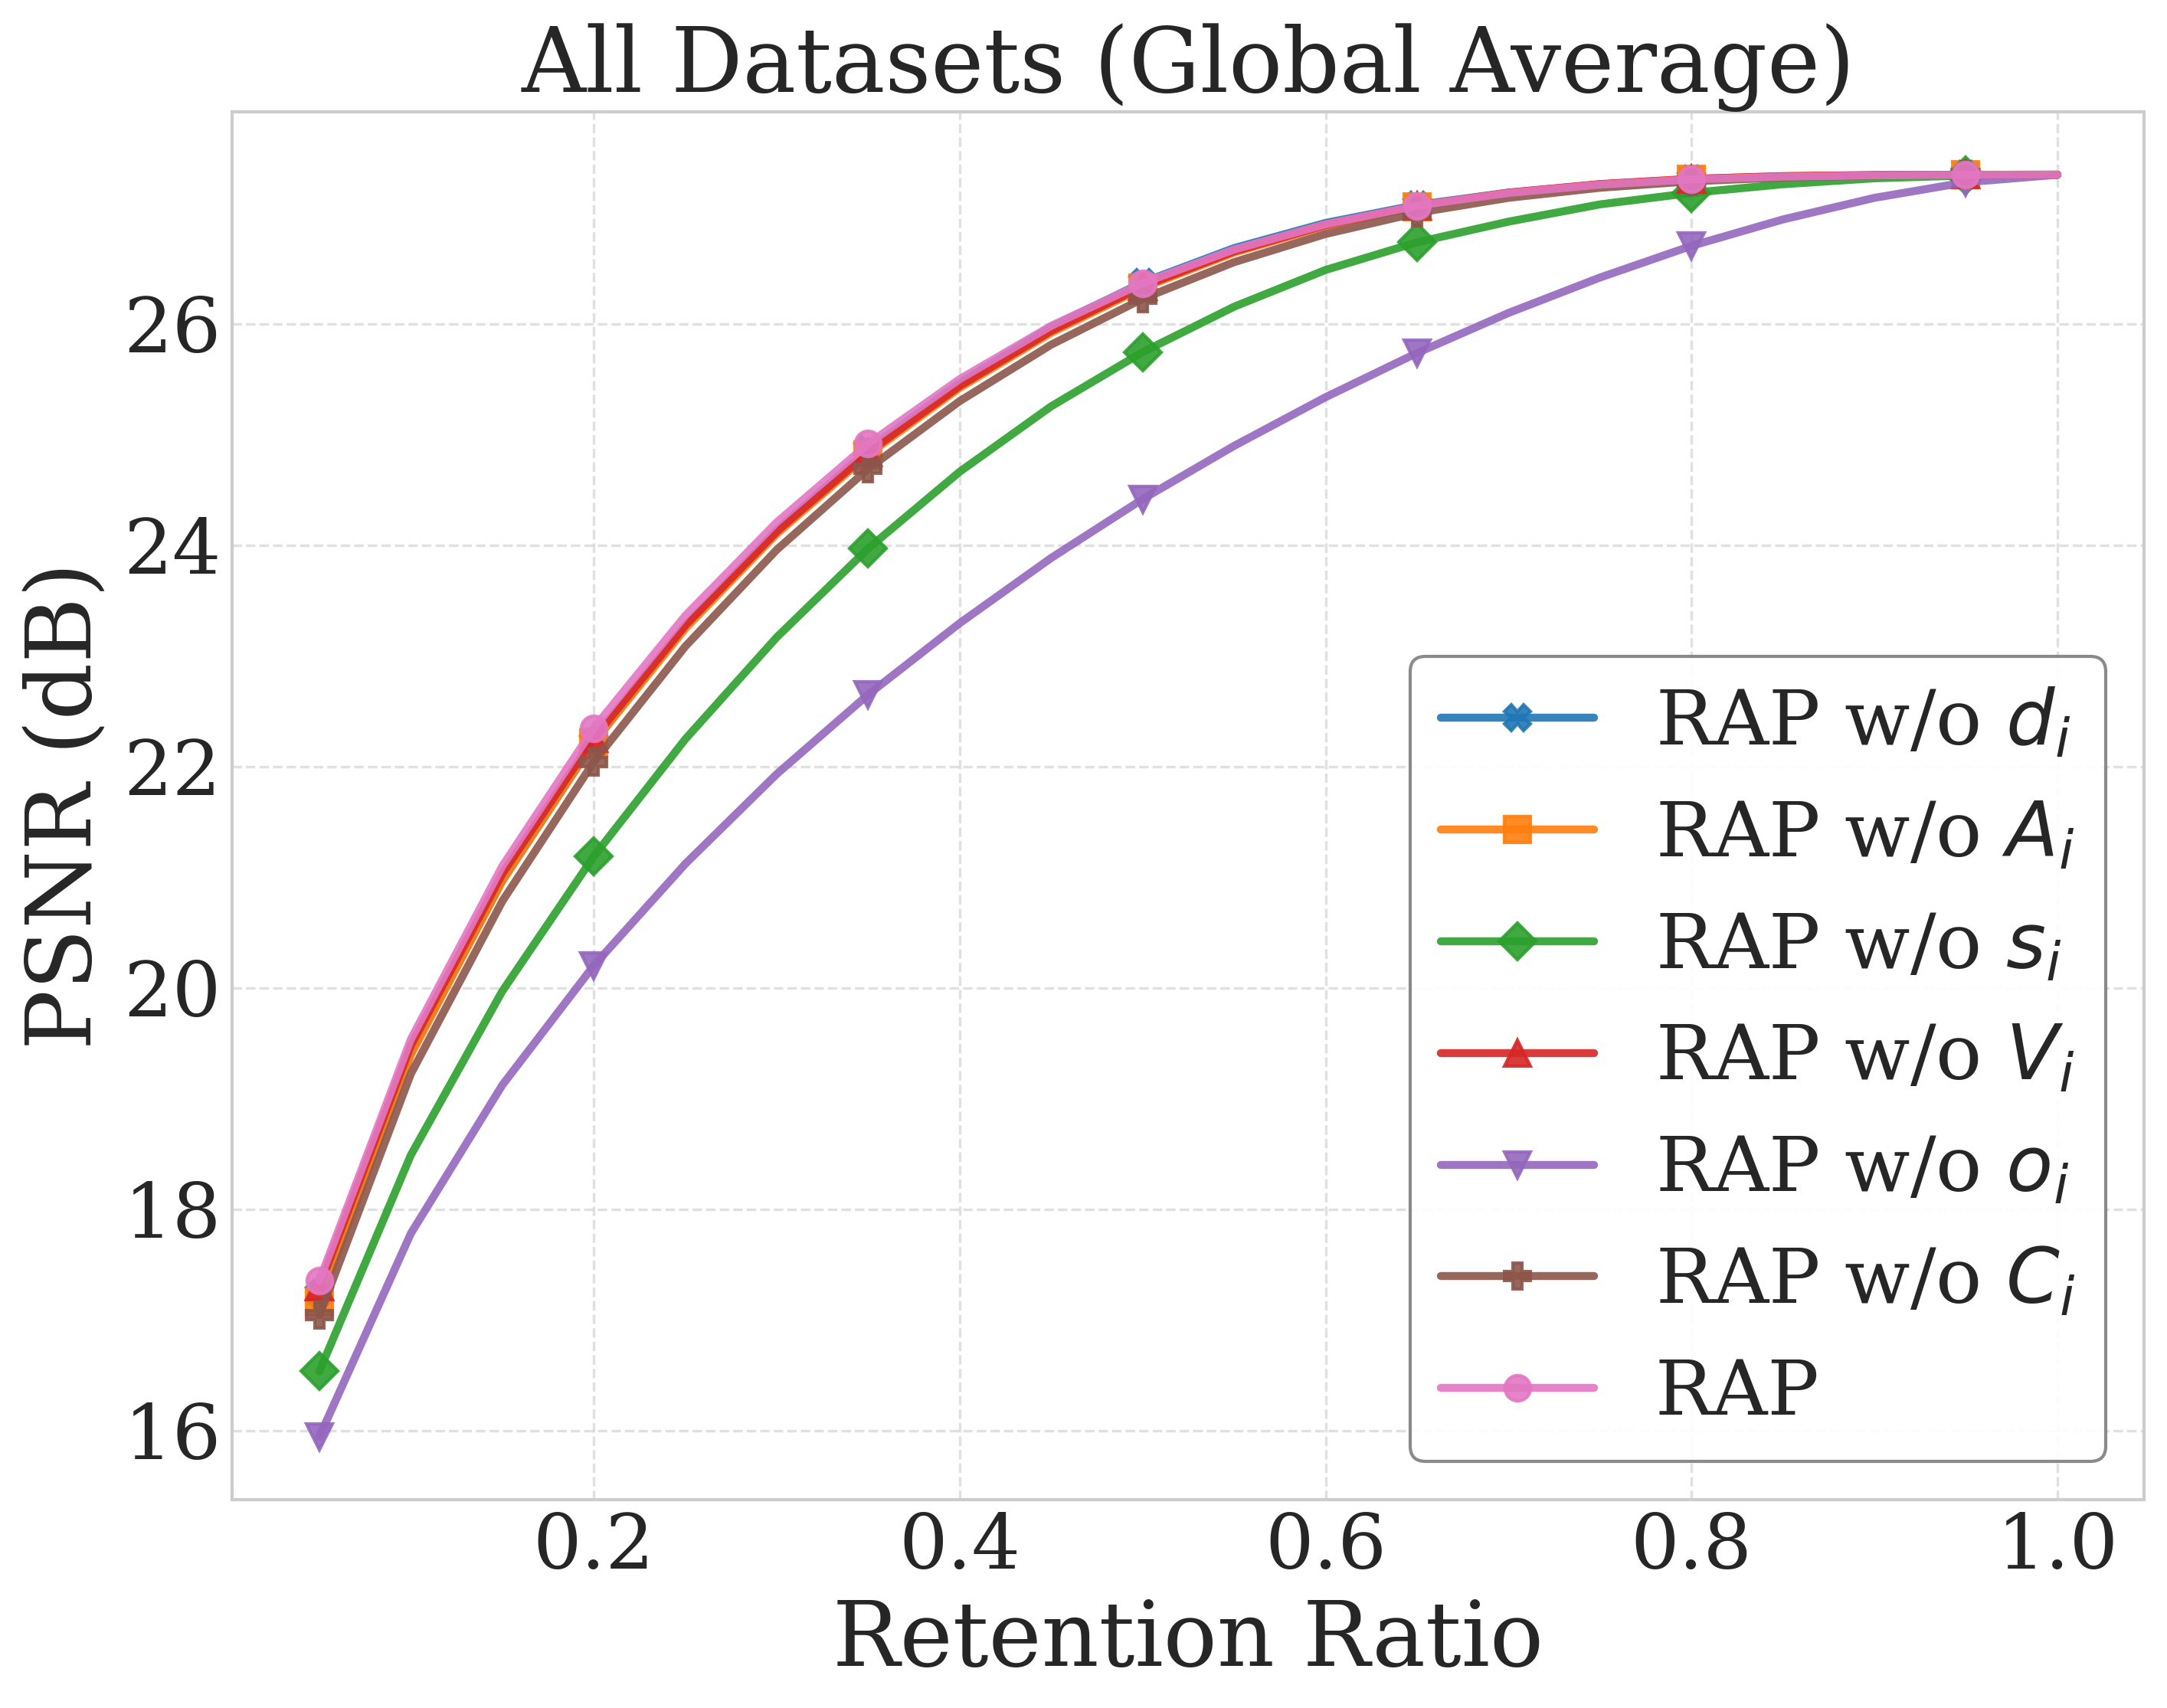
\includegraphics[width=\linewidth]{sec/imgs_main/abla_feature1_avg.png}
    \caption{Individual features}
    \label{fig:abla_feat1}
  \end{subfigure}
  \hfill
  \begin{subfigure}{0.48\linewidth}
    \centering
    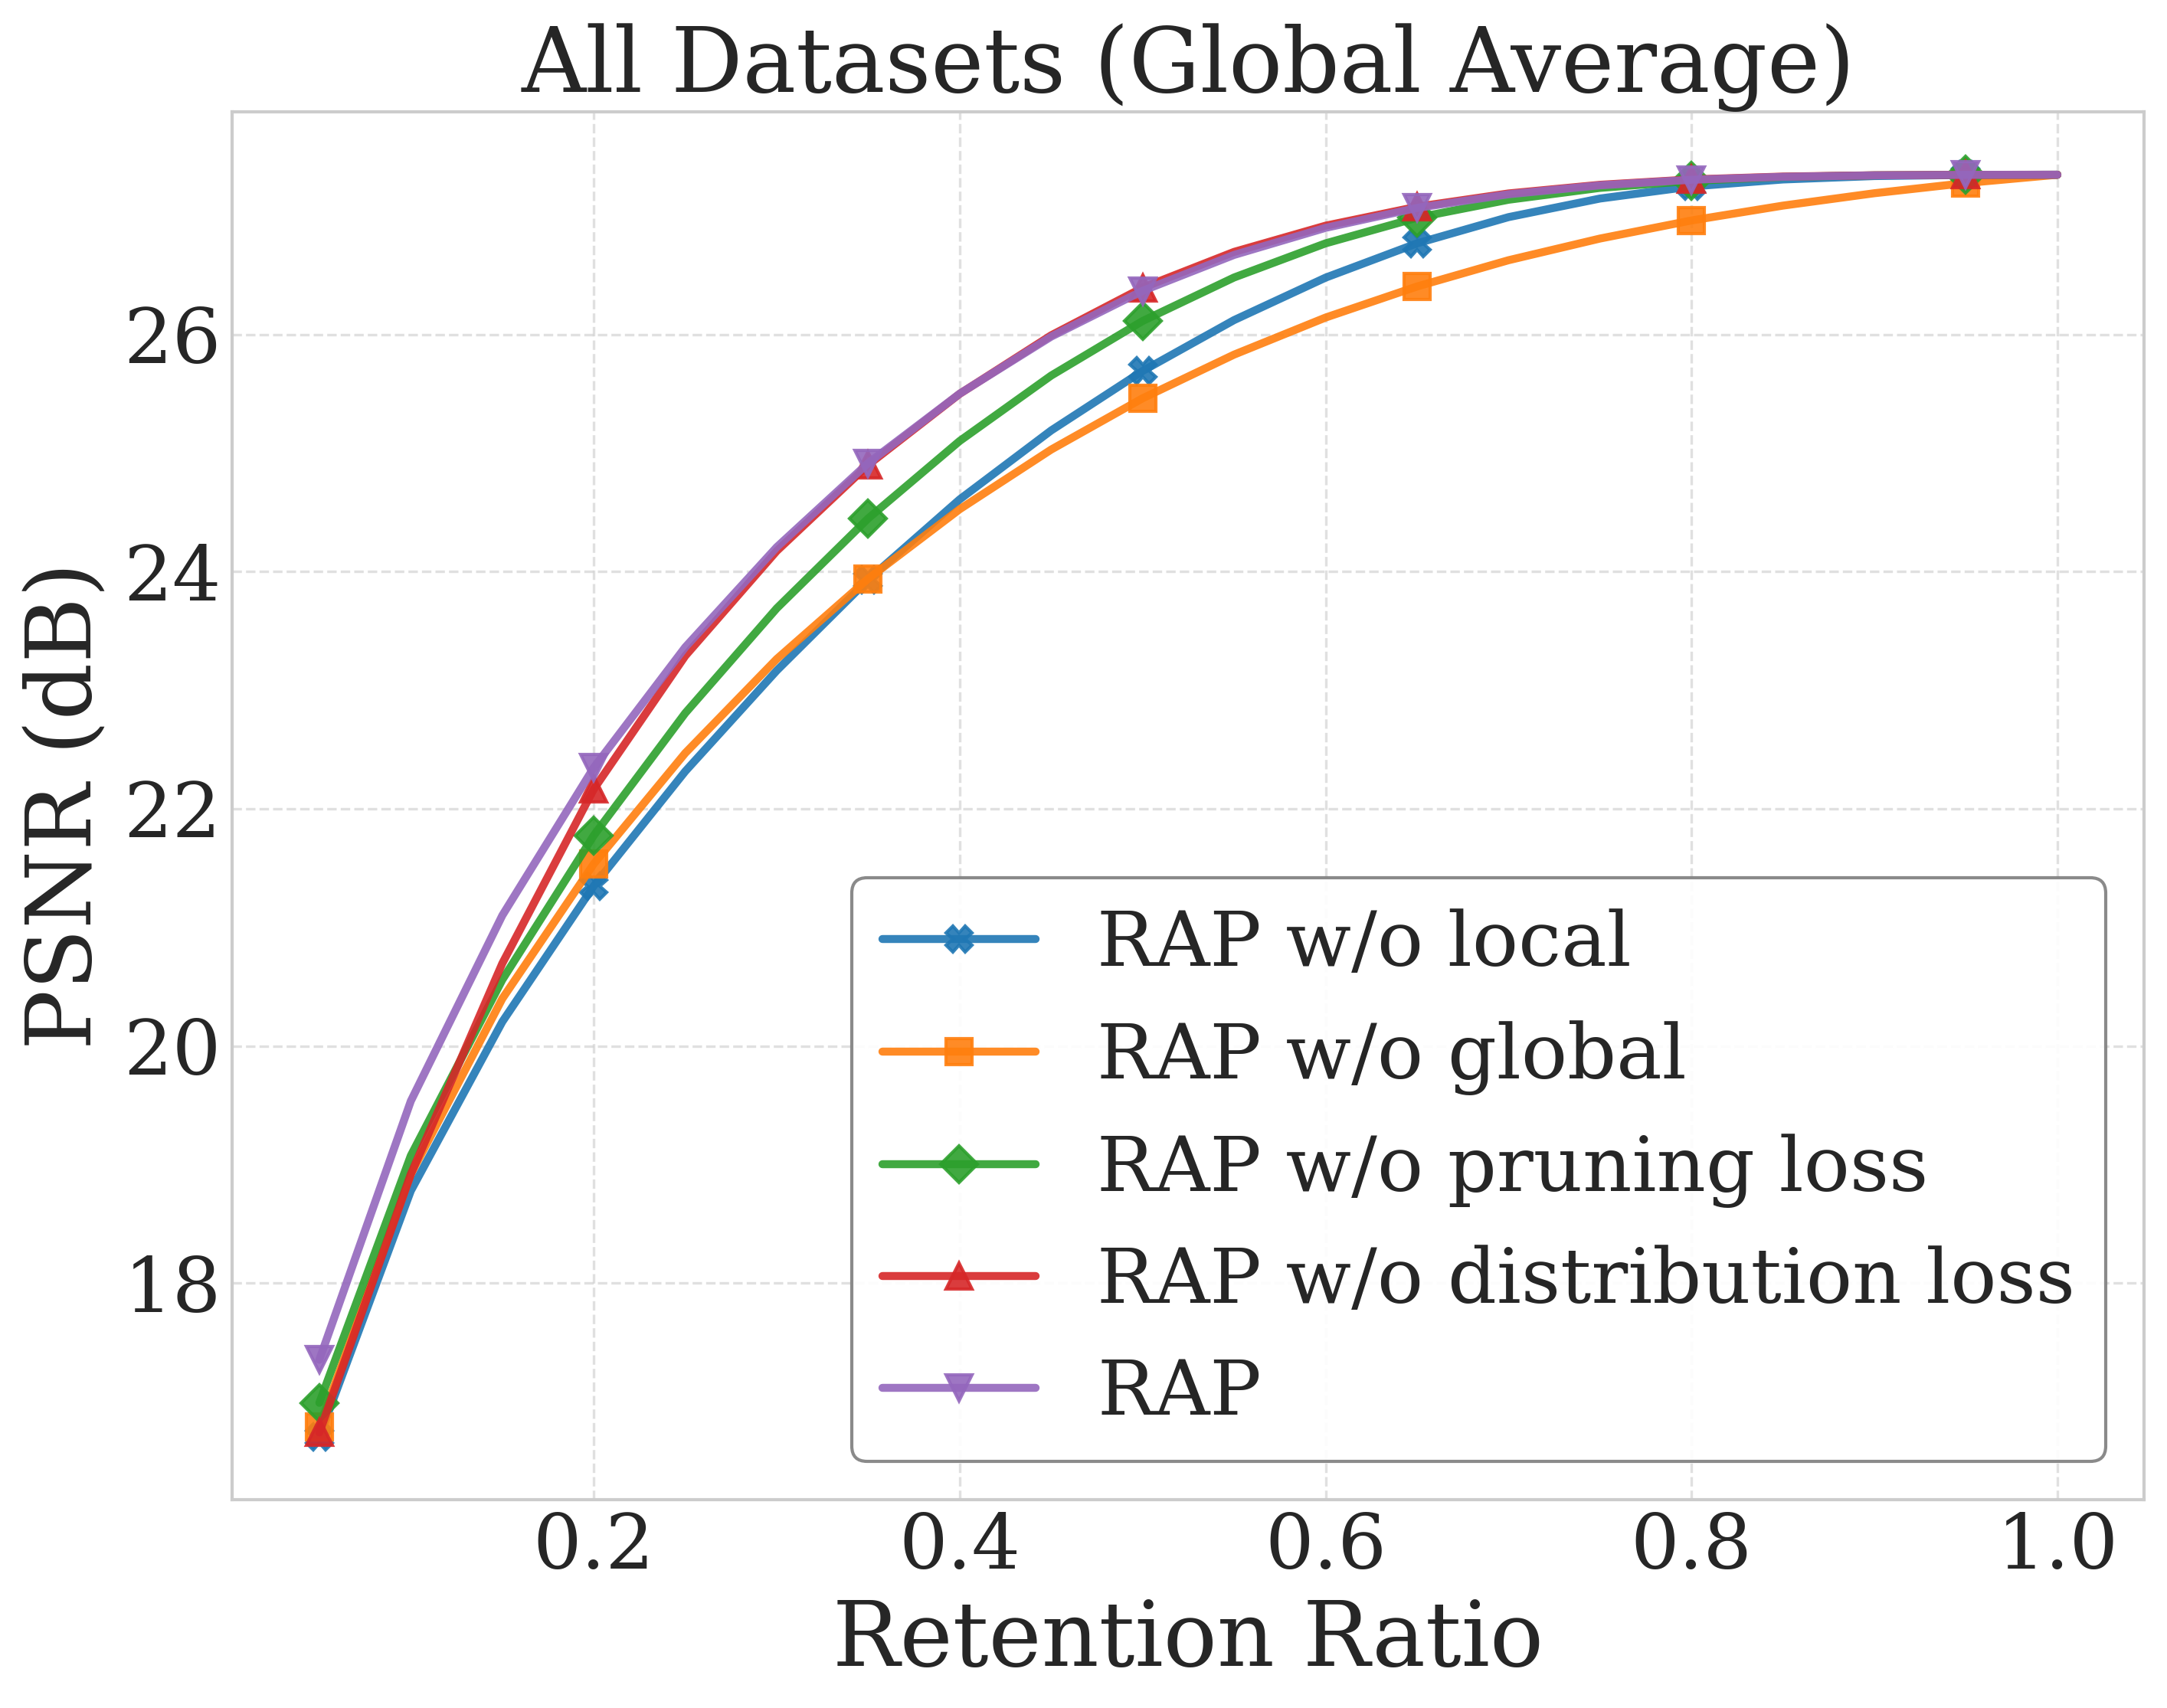
\includegraphics[width=\linewidth]{sec/imgs_main/abla_feature2_loss_avg.png}
    \caption{Normalization and loss}
    \label{fig:abla_feat2}
  \end{subfigure}

  \caption{
    Ablation studies of the proposed feature and loss.
  }
  \label{fig:abla_half}
  \vspace{-1.5em}
\end{figure}
To better understand the behavior and design choices of RAP, we conduct comprehensive ablation studies feature effectiveness and loss formulation.
We perform a series of experiments to analyze two aspects: 
(1) the effectiveness of the proposed feature design and normalization strategy; and 
(2) the contribution of each loss term in our RAP training.

$\bullet$\textbf{Effectiveness of feature design.}
As formulated in Equation~\ref{equ:feature}, RAP integrates geometric and appearance descriptors 
$\{d_i, A_i, s_{0,i}, s_{1,i}, s_{2,i}, V_i, o_i, C_i\}$ 
together with their local and global normalized counterparts.
To assess the contribution of each component, we perform two ablation experiments.

Fig.~\ref{fig:abla_feat1} evaluates the contribution of each feature by removing one attribute at a time while keeping all others unchanged. Opacity $o_i$ proves to be the most crucial cue—its removal leads to about 1-2~dB PSNR drop at the same pruning ratio. 
Gaussian scales $\{s_{0,i}, s_{1,i}, s_{2,i}\}$ follow as the next most influential features, causing around 0.5–1~dB degradation when excluded. 
Other features, including color anisotropy $A_i$ and average KNN distance $d_i$, provide smaller yet consistent benefits, particularly at aggressive pruning ratios, indicating their complementary role. 

$\bullet$\textbf{Normalization and loss formulation.}
Fig.~\ref{fig:abla_feat2} analyzes the effect of normalization and loss design.  
Removing either local or global normalization leads to a substantial PSNR drop (1.5--2~dB), confirming their complementary roles: 
local normalization enhances intra-region contrast to better separate redundant primitives, 
while global normalization ensures scene-level consistency and stabilizes feature magnitudes across datasets. 
Together, they support robust and generalizable importance estimation under diverse scene conditions.

The pruning-aware loss also plays a critical role. 
Removing it results in a moderate but consistent degradation (around 0.5~dB on average), as the network loses explicit control over the expected pruning ratio. 
As visualized in the supplementary material (Sec.~\ref{sup:loss}), the absence of this loss causes the predicted score distribution to shift toward a higher mean, reflecting overly conservative pruning.

The distribution loss contributes smaller yet steady improvements, with a noticeable gain at low retention ratios (approximately 0.25~dB). 
This effect is most evident in dense and complex scenes, where enforcing a smooth score distribution helps differentiate subtle importance variations among overlapping primitives. 
Without this loss, the predicted scores collapse toward near-binary outputs around 0 and~1 (see Sec.~\ref{sup:loss}), reducing the model's flexibility to support arbitrary pruning ratios.
